\documentclass[12pt]{report}

%\usepackage[a4paper, left = 2.5cm, top = 2.5cm, bottom = 2cm, right = 2cm]{geometry}

\usepackage{vmargin}

\setpapersize{A4}
\setmargins{2.5cm}       % margen izquierdo
{2.5cm}                  % margen superior
{16.5cm}                 % anchura del texto
{23.42cm}                % altura del texto
{10pt}                   % altura de los encabezados
{1cm}                    % espacio entre el texto y los encabezados
{0pt}                    % altura del pie de página
{2cm}                    % espacio entre el texto y el pie de página



\usepackage[spanish,es-tabla]{babel} % Idioma español con tablas
\usepackage{longtable}     % Usado para diseñar grandes tablas.
\usepackage{multirow} % para las tablas

\usepackage{amsmath, amssymb, amsfonts, latexsym, anyfontsize}
\usepackage{color, alltt, times}
\setcounter{secnumdepth}{3} %para que ponga 1.1.1.1 en subsubsecciones
\setcounter{tocdepth}{3}    % para que ponga subsubsecciones en el indice
\usepackage{setspace}       % Usado para %\onehalfspace  \doublespacing  \singlespace
\usepackage{booktabs}       % Para formar tablas
\usepackage{appendix}       % para los anexos
\usepackage{url}            % para citar las urls
\usepackage{pdfpages}       % para insertar documentos de tipo PDF
\usepackage{epstopdf}       % para insertar imagenes en formato eps obtenidas en Matlab
\usepackage{graphicx}       % para las imagenes y gráficos
\usepackage{subfigure}      % para subfiguras

\usepackage[utf8]{inputenc}         % Para escribir en castellano
\usepackage[T1]{fontenc}

\usepackage{algorithmic}
\usepackage{algorithm}
\floatname{algorithm}{Algoritmo}
\renewcommand{\listalgorithmname}{Lista de algoritmos}
\renewcommand{\algorithmicrequire}{\textbf{Entrada:}}
\renewcommand{\algorithmicensure}{\textbf{Salida:}}
\renewcommand{\algorithmicend}{\textbf{FIN}}
\renewcommand{\algorithmicif}{\textbf{SI}}
\renewcommand{\algorithmicthen}{\textbf{ENTONCES}}
\renewcommand{\algorithmicelse}{\textbf{CASO CONTRARIO}}
\renewcommand{\algorithmicelsif}{\algorithmicelse,\ \algorithmicif}
\renewcommand{\algorithmicendif}{\algorithmicend\ \algorithmicif}
\renewcommand{\algorithmicfor}{\textbf{PARA}}
\renewcommand{\algorithmicforall}{\textbf{para todo}}
\renewcommand{\algorithmicdo}{\textbf{HACER}}
\renewcommand{\algorithmicendfor}{\algorithmicend\ \algorithmicfor}
\renewcommand{\algorithmicwhile}{\textbf{MIENTRAS}}
\renewcommand{\algorithmicendwhile}{\algorithmicend\ \algorithmicwhile}
\renewcommand{\algorithmicloop}{\textbf{REPETIR}}
\renewcommand{\algorithmicendloop}{\algorithmicend\ \algorithmicloop}
\renewcommand{\algorithmicrepeat}{\textbf{REPETIR}}
\renewcommand{\algorithmicuntil}{\textbf{HASTA}}
\renewcommand{\algorithmicprint}{\textbf{imprimir}} 
\renewcommand{\algorithmicreturn}{\textbf{RETORNAR}} 
\renewcommand{\algorithmictrue}{\textbf{cierto }} 
\renewcommand{\algorithmicfalse}{\textbf{falso }} 
 % mi archivo de traducción

\usepackage[x11names,table]{xcolor}


\usepackage[round]{natbib} 
 
\graphicspath{ {images/} }
\begin{document}


\baselineskip 1cm
\pagestyle{plain}
%%%%%%%%%%%%%%%%%%%%%%%%%%%%% CARATULA%%%%%%%%%%%%%%%%%%%%%%%%
\textheight 19cm
\pagestyle{empty}
\begin{center}
 {\bf {\fontsize{14}{16.8}\selectfont UNIVERSIDAD NACIONAL DE TRUJILLO}}     
 
    {\bf{\fontsize{14}{16.8}\selectfont Facultad de Ciencias Físicas y Matemáticas}} 

  {\bf{\fontsize{14}{16.8}\selectfont Escuela Profesional de Informática}}
\end{center}  

\begin{figure}[ht]
\begin{center}

\includegraphics[width=.4\textwidth]{unt}
\end{center}
\end{figure}

\vskip 2cm
\begin{center}
  { \bf {\fontsize{17}{20.4}\selectfont{MODELO PARA LA RUTERIZACIÓN }}     
  \vskip 3cm
  %{\hspace{-1.7cm}AUTOR(ES):}\par
  {\bf \fontsize{14}{16.8}\selectfont {\hspace{-2.9cm}AUTOR(ES): José Vicente Clavo Tafur}}} \\
    \vskip 0.2cm
    {\bf \fontsize{14}{16.8}\selectfont {\hspace{-1.7cm} ASESOR: Gutierrez}}

     
\end{center}   


\vskip 1.1cm
\begin{center}    
{\bf {\fontsize{14}{16.8}\selectfont Trujillo - Perú
\vskip 0.0cm
\hspace*{-0.2cm} 
2019 }}
\end{center} 
\newpage
%%%%%%%%%%%%%%%%%%%%%%%%%%%%%%%%%%%%%%%%%%%%%%%%%%%%%%%%%%%%%%%%%%%%%%%%%%%


%%%%%%%%%%%%%%%%%%%%%%%%%%%%CONTRA CARATULA 1 %%%%%%%%%%%%%%%%%%%%%%%%%%%%%
\newpage
\pagestyle{plain}
\pagenumbering{roman}

\hspace*{6cm}
\vskip 9cm
\begin{center}
   {\bf \doublespacing {\fontsize{17}{20.4}\selectfont{PREDICCIÓN DE LA RESPUESTA CORRECTA DE UNA PREGUNTA DE OPCIÓN MÚLTIPLE MEDIANTE TÉCNICAS DE APRENDIZAJE NO SUPERVISADO ASOCIADO CON LA EXPERIENCIA.}}}     
\end{center} 
\newpage
%%%%%%%%%%%%%%%%%%%%%%%%%%%%%%%%%%%%%%%%%%%%%%%%%%%%%%%%%%%%%%%%%%%%%%%%%%%


%%%%%%%%%%%%%%%%%%%%%%%%%%%%% CONTRA CARATULA 2 %%%%%%%%%%%%%%%%%%%%%%%
\begin{center}
   {\bf {\fontsize{14}{16.8}\selectfont{José Vicente Clavo Tafur}}}\\     
   \end{center}   

\vskip 3.2cm
\begin{center}
   {\bf \doublespacing {\fontsize{17}{20.4}\selectfont{PREDICCIÓN DE LA RESPUESTA CORRECTA DE UNA PREGUNTA DE OPCIÓN MÚLTIPLE MEDIANTE TÉCNICAS DE APRENDIZAJE NO SUPERVISADO ASOCIADO CON LA EXPERIENCIA.}}}     
\end{center}   
  \vskip 2cm
\begin{verse}
 \fontsize{12}{14.4}\selectfont{\hspace*{0.6cm}Tesis presentada a la Escuela Profesional de Informática en la Facultad de Ciencias Físicas y Matemáticas de la Universidad Nacional de Trujillo, como requisito parcial para la obtención del grado de Bachiller en ciencia de la computación ( Título profesional de Ing. Informático)}
\end{verse}

\vskip 1.5cm 
{\fontsize{14}{16.8}\selectfont ASESOR: JOSÉ A. RODRIGUEZ MELQUIADES} 
 \vskip 1cm 
 \begin{center}    
 \vskip 2cm
{\fontsize{14}{16.8}\selectfont Trujillo - Perú
\vskip 0.2cm
\hspace*{-0.2cm} 
2019}
\end{center} 
\newpage
%%%%%%%%%%%%%%%%%%%%%%%%%%%%%%%%%%%%%%%%%%%%%%%%%%%%%%%%%%%%%%%%%%%%%%%%%%%%%


%%%%%%%%%%%%%%%%%%%%%%%%%%%%HOJA DE APROBACION %%%%%%%%%%%%%%%%%%%%%%%%%%%%%
\begin{center}
 {\bf {\Large HOJA DE APROBACIÓN }     
 \vskip 1.5cm
  {\Large PREDICCIÓN DE LA RESPUESTA CORRECTA DE UNA PREGUNTA DE OPCIÓN MÚLTIPLE MEDIANTE TÉCNICAS DE APRENDIZAJE NO SUPERVISADO ASOCIADO CON LA EXPERIENCIA.}}
 \vskip 1cm 
  {\large{José Vicente Clavo Tafur}}\\

 \vskip 1cm
\end{center} 
Tesis defendida y aprobada por el jurado examinador:
\vskip 1.5 cm
\begin{flushleft} 
$\overline{\mbox{Prof. Dr. XXXXXX - Asesor}}$\\
\vskip -0.5cm
Departamento de Informática - UNT
\end{flushleft} 
\vskip 1cm
\begin{flushleft} 
$\overline{\mbox{Prof. Mg. XXXXXX}}$\\
\vskip -0.5cm
Departamento de Informática - UNT
\end{flushleft} 
\vskip 1cm
\begin{flushleft} 
$\overline{\mbox{Prof. Mg. XXXXXXX}}$\\
\vskip -0.5cm
Departamento de Informática - UNT
\end{flushleft}
\vskip 0.8cm 
\begin{center}    
Trujillo, xX de mayo del 2019
\end{center} 
\newpage
%%%%%%%%%%%%%%%%%%%%%%%%%%%%%%%%%%%%%%%%%%%%%%%%%%%%%%%%%%%%%%%%%%%%%%%%%%%%


%%%%%%%%%%%%%%%%%%%%%%%%%%%% DEDICATORIA %%%%%%%%%%%%%%%%%%%%%%
 
 \addcontentsline{toc}{chapter}{Dedicatoria}
 {\bf\Large {Dedico esta tesis a :}}
 \vskip 1cm
\begin{quotation}
{\it Mis padres quienes en todo momento me apoyaron. En especial a mi madre quien fue mi motor para seguir en mi camino y poder finalizar este proyecto.
\vskip 1cm
Mi hermano con quien siempre compartimos conocimiento para así poder re-solver algunos problemas que aparecieron en el transcurso del desarrollo de este proyecto.
\vskip 1cm
A todas las personas que contribuyen con las ciencia en el Perú y cada día se esfuerzan para que esta siga creciendo }
\end{quotation}
%%%%%%%%%%%%%%%%%%%%%%%%%%%%%%%%%%%%%%%%%%%%%%%%%%%%%%%%%%%%%%%%%%%%%%%%%%%


%%%%%%%%%%%%%%%%%%%%%%%%%%%% AGRADECIMENTOS %%%%%%%%%%%%%%%%%%%%%%
\newpage

 \addcontentsline{toc}{chapter}{Agradecimientos}
 {\bf\Large {\flushleft{Agradecimientos}}}
 \vskip 1.5cm
\begin{quotation}
Agradezco a Dios por haberme bendecido en toda mi vida ....
{\vskip 1cm}
A mis profesores del Departamento de Informática, de los cuales recibí una gran cantidad de conocimientos  . 
\vskip 1cm
A  mi  asesor  Prof.  Dr.  José  Luis  Gutierrez Gutierrez  que  siempre  se  mostró disponible e interesado en ayudarme.
\vskip 1cm
 . . .
 \end{quotation}
%%%%%%%%%%%%%%%%%%%%%%%%%%%%%%%%%%%%%%%%%%%%%%%%%%%%%%%%%%%%%%%%%%%%%%%%%%%


%%%%%%%%%%%%%%%%%%%%%%%%%%%% RESUMEN%%%%%%%%%%%%%%%%%%%%%%
\newpage
\begin{center}
 \addcontentsline{toc}{chapter}{Resumen}
 {\bf\LARGE Resumen}
\end{center} 
\vskip 0.5cm
\begin{quotation}
{\bf Ejemplo:}\par

En la actualidad, hay algunas evaluaciones que son aplicadas en una determina-da fecha y los resultados no son entregadas hasta algunos meses después, creando un ambiente de incertidumbre acerca de los resultados. Estas son evaluaciones que constan  de  preguntas  tipo  opción  múltiple  las  cuales  requieren  de  conocimiento académicos previos para poder responder correctamente. Por ejemplo una evaluación con esas características son las evaluaciones que miden el nivel en un idioma extranjero  como  puede  ser  el  Inglés  (ECCE,MET,etc).  En  este  caso  los  resultados de estas evaluaciones son entregadas 2 meses después de haber sido aplicadas.
\vskip 0.2cm 
Esta investigación tiene como objetivo principal la predicción de la respuesta correcta de las preguntas de este tipo de evaluaciones. Para ello se usaran técnicas de aprendizaje no supervisado (Algoritmo K-means) asociado con la experiencia previa. Como experiencia previa se usará las calificaciones anteriores obtenidas delos 2 últimos exámenes de los estudiantes. Los resultados muestran que es posible estas predicciones mostrando un porcentaje de acierto de XX \%   

\vskip 0.3cm
\hspace*{-0.6cm}{\bf Palabras claves:} predicción, clusters, respuesta correcta, aprendizaje no supervisado.
\end{quotation}
%%%%%%%%%%%%%%%%%%%%%%%%%%%%%%%%%%%%%%%%%%%%%%%%%%%%%%%%%%%%%%%%%%%%%%%%%%%%%%%%%%%%


%%%%%%%%%%%%%%%%%%%%%%%%%%%%ABSTRACT%%%%%%%%%%%%%%%%%%%%%%
\newpage
\begin{center}
 \addcontentsline{toc}{chapter}{Abstract}
 {\bf\LARGE Abstract}\vskip 1.5cm
\end{center} 
\begin{quotation}

{\bf Ejemplo:}\par

Nowadays, There are some tests which are taken in a specific date and their results are showed some month later. It creates a state of uncertainty about the results. These are tests which have multiple choice questions and previous knowledge is required to solve them. For example, a test with these characteristic is the test to measure the English level such as MET, ECCE and others. For these exams thei rresults are showed two months later. 
\vskip 0.2cm
The main goal of this research is the prediction of the right answer of a multiplechoice question. To get this objective unsupervised learning algorithms (K-means)linked with previous experience will be used. In this case the previous experiencewill be the two last student’s grades.
The outcomes of this research show XX \% right so these predictions are correct.
\vskip 0.3cm
\hspace*{-0.6cm}{\bf Keywords:} prediction, cluster, rigth answer, unsupervised learning.
\end{quotation}
%%%%%%%%%%%%%%%%%%%%%%%%%%%%%%%%%%%%%%%%%%%%%%%%%%%%%%%%%%%%%%%%%%%%%%%%%%%%%%


%%%%%%%%%%%%%%%%%%%%%%%%%%% LISTA DE SIMBOLOS %%%%%%%%%%%%%%%%%%%%%%
\newpage
\addcontentsline{toc}{chapter}{Lista de símbolos}
 {\bf\LARGE Lista de símbolos}
 \vskip 1.5cm
Constantes: 
\begin{enumerate}
\item[(1)]$r,\overline{r} $ \hspace*{0.8cm} Indice que denota regiones.
\item[(2)] $n $ \hspace*{1.1cm} Indice de bienes finales deseados por los consumidores.
\item[(3)] ...
\vskip 3cm
\end{enumerate} 
\vskip 0.3cm
Variables:
\begin{enumerate}
\item[(5)] $ x^{r} $ \hspace*{1cm} Vector columna que denota la actividad de producción.
\item[(6)] $ u^{r} $ \hspace*{1.2cm} . . .
\end{enumerate}

              % Datos de la tesis
\listoffigures               % indice de figuras
\addcontentsline{toc}{chapter}{Índice de Figuras}
\listoftables                % indice de tablas
\addcontentsline{toc}{chapter}{Índice de Tablas}
\tableofcontents             % indice de materias
\chapter{Introducción}
\pagenumbering{arabic}
\setcounter{page}{1}
%\renewcommand{\baselinestretch}{2} %doble espacio paratodo el texto
%\renewcommand{\baselinestretch }{1.5}
 
En esta investigación se realizará la predicción de la respuesta correcta de una pregunta de opción múltiple, este tipo de pregunta de una evaluación requiere de conocimiento previo para ser respondida, mediante técnicas de aprendizaje no supervisado asociado con la experiencia previa. Como experiencia previa se usará las calificaciones anteriores obtenidas de los 2 últimos exámenes de los estudiantes.
\vskip 0.3cm
Para ello se plantea desarrollar un algoritmo de aprendizaje automático no supervisado llamado K-means, el cual sirve para crear clusters. Estos clusters se formarán con la data de las calificaciones  anteriores  de  los  estudiantes. Así  se  obtendría  un  valor  promedio,  Además,  se utilizará técnicas de estadísticas para crear un histograma de las opciones de las preguntas respondidas. Combinando estas 2 técnicas se obtendría una predicción por cada pregunta.
\vskip 0.3cm  
Este proyecto fue pensado debido a la problemática que se tiene al aplicar una evaluación y tener que esperar demasiado tiempo para obtener las respuestas correctas. Pero con lo que se desarrollara se obtendrá la respuesta correcta en corto tiempo.
\vskip 0.3cm 
Para cumplir los objetivos de este proyecto se tendrá primero que investigar acerca del aprendizaje automático no supervisado, así como las teorías de la probabilidad. Luego se desarrollará el algoritmo de aprendizaje automático no supervisado; ya hecho esto se procederá al desarrollo del prototipo de software web para poder ingresar los datos y hacer las pruebas. Finalmente se documentarán los resultados obtenidos.

\section{Justificación de la investigación}
La investigación es justificada por lo siguiente:   

\begin{enumerate}
\item[(a)] En esta investigación pondremos en practica técnicas de aprendizaje de máquinas no supervisado, además se utilizará teorías de predicción para poder llevar acabo su objetivo. 

\item[(b)]Esta investigación permitirá a los estudiantes tener un predicción del resultado de su examen en corto tiempo y así tener una idea de como sera su resultado. Además los educadores podrán usar esta información para la toma de decisiones.

\item[(c)]Los resultados de la investigación presentarán cómo resultado esperado, un prototipo de software que permita predecir la respuesta correcta de las pregunta de la evaluación. Este prototipo de software usará un algoritmo de aprendizaje no supervisado para trabajar con la información previa de los estudiantes (sus calificaciones anteriores).
\end{enumerate}


\section{Formulación del problema}

  En este trabajo, se propone responder a la siguiente pregunta:
 \begin{center} 
     ¿ Cómo predecir la respuesta correcta de una pregunta de opción múltiple?
 \end{center}


\section{Hipótesis}
Mediante el desarrollo de un algoritmo de aprendizaje no supervisado y experiencia previa, se puede predecir la respuesta correcta de una pregunta de opcion multiple. \par  
\vskip 0.3cm

\section{Objetivos}

\subsection{Generales}
\begin{enumerate}
\item[a)] Desarrollar un algoritmo de aprendizaje no supervisado para predecir la respuesta correcta de una pregunta de opción múltiple.
\end{enumerate}

\subsection{Específicos}
\begin{enumerate}
\item[a)] Codificar el algoritmo de aprendizaje no supervisado para trabajar con clusters.
\item[b)] Desarrollar del prototipo de software y aplicarla a la predicción de la respuesta correcta.
\item[c)] Realizar las pruebas y documentar resultados.
\end{enumerate}
\vskip 0.3cm


\section{Estructura de la tesis}

\vskip 0.1cm
El presente trabajo está dividido en cinco capítulos. El primer capítulo presenta los aspectos generales del tema tratado: justificación de la investigación, formulación del problema, hipótesis, objetivos y la estructura de la tesis.

En el segundo capítulo se contempla el marco teórico donde se hace referencia a los conceptos de predicción, pregunta de opción múltiple y de prototipo de software, además se hace referencia a la metodología de la investigación.

El tercer capítulo trata del tema central de la tesis, diseñándose el algoritmo K-means, se muestra el proceso para hacer la predicción y como se desarrolló el prototipo de aplicación web.

En el cuarto capítulo se presentan los resultados obtenidos en la investigación. 

En el quinto capitulo se presentan las conclusiones, seguidas de las recomendaciones para futuras investigaciones relacionadas al tema en cuestión. 

Finalmente las referencias bibliográficas usadas para la investigación. Además de los apéndices donde se presenta el algoritmo elaborado, los datos de los resultados y los instrumentos usados para recoger información.

\chapter{Materiales y métodos}

En este capítulo se explica cual fue la metodología empleada para la solución del problema formulado, además de una reseña del material bibliográfico investigado con relación a los temas considerados en esta investigación. Los conocimientos investigados son muy amplios, principalmente los que ayudaron a consolidar las bases del conocimiento científico para elaborar esta tesis, como lo son los temas de ******************************************* FALTA COMPLETAR
%\vskip 1cm 


\section{Marco teórico}
\subsection{Aprendizaje no supervisado}

\subsubsection{Definición}

Aprendizaje no supervisado es un método de adiestramiento automático donde un modelo es ajustado a las observaciones. Se distingue del  aprendizaje supervisado por el hecho de que no hay un conocimiento a priori. En el aprendizaje no supervisado, un conjunto de datos de objetos de entrada es tratado. Así, el aprendizaje no supervisado típicamente trata los objetos de entrada como un conjunto de variables aleatorias, siendo construido un modelo de densidad para el conjunto de datos.
\vskip 1cm
En este método contamos con “objetos” o muestras, que tiene un conjunto de características, de las que no sabemos a que clase o categoría pertenece, entonces la finalidad es el descubrimiento de grupos de “objetos” cuyas características afines nos permitan separar las diferentes clases \citep{Araujo}.

\subsubsection{Características}

En este apartado se muestran las principales características del método de aprendizaje no supervisado. \citep{Hinton_Sejnowski}.

\begin{itemize}
\item No necesitan de un profesor externo.
\item Muestran cierto grado de auto-organización.
\item La red descubre en los datos de entrada y de forma autónoma: características, regularidades, correlaciones y categorías.
\item Suelen requerir menores tiempos de entrenamiento que las supervisadas.
\item Abordan los siguientes tipos de problemas: familiaridad, análisis de componentes principales, agrupamiento y relación de características.
\end{itemize}

\subsubsection{Técnicas}
Existen diferentes técnicas para el método de aprendizaje no supervisado.

\begin{description}
	\item[Clustering:] Agrupan objetos en regiones donde la similitud mutua es elevada.
	\item[Visualización:] Permiten observar la amplitud de instancias en un espacio de menor dimensión.
	\item[Reducción de la dimensionalidad:] Los datos de entrada son agrupados en subespacios de una dimensión más baja que la inicial.
	\item[Extracción de características:] construyen nuevos atributos (pocos) a partir de los originales (muchos).
\end{description}


\subsection{Clustering}

\subsubsection{Definición}

Análisis de grupo o agrupamiento (en inglés, clustering) es un procedimiento de agrupación de una serie de vectores de acuerdo con un criterio. Esos criterios son por lo general distancia o similitud. La cercanía se define en términos de una determinada función de distancia, como la euclídea. La medida más utilizada para medir la similitud entre los casos es la matriz de correlación entre los \( N x N \) casos.
\vskip 1cm
Generalmente, los vectores de un mismo grupo o clúster comparten propiedades comunes. El conocimiento de los grupos puede permitir una descripción de un conjunto de datos multidimensional complejo. Esta descripción se consigue sustituyendo el detalle de todos los elementos de un grupo por la de un representante característico del mismo.

\begin{figure}[ht]
	\begin{center}
		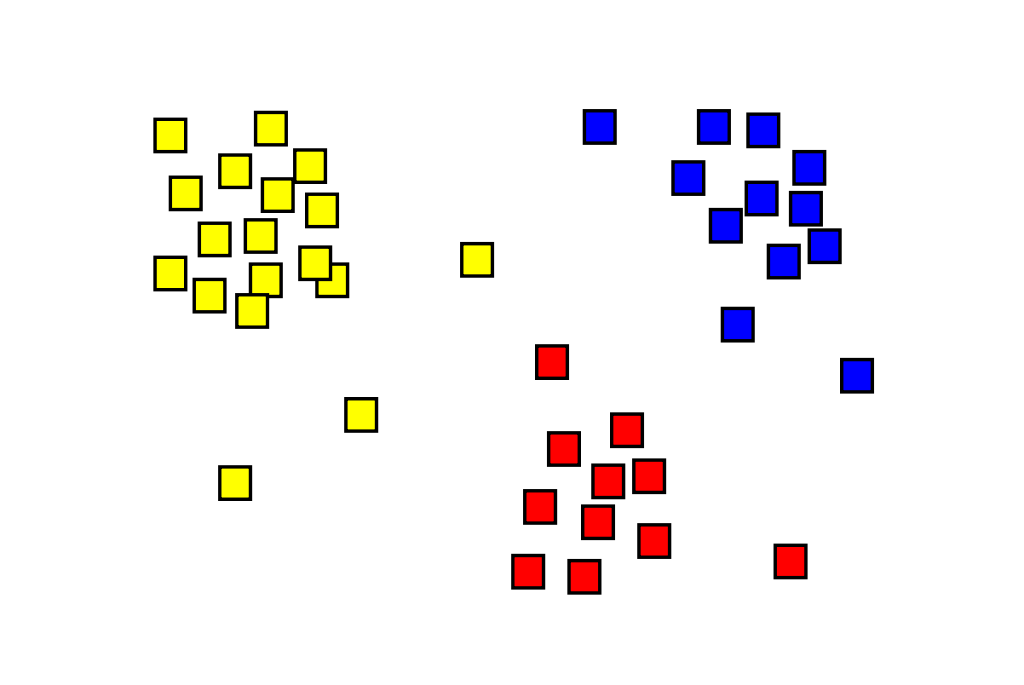
\includegraphics[width=0.3\textwidth]{clustering}
	\end{center}
	\begin{center}
		\vskip -0.5cm
		\caption{\small{El resultado de un análisis de grupo, mostrado como la coloración de cuadrados en tres grupos.}}
		{\small{Fuente: }}
	\end{center}
\end{figure}

Clustering es considerado una técnica de aprendizaje no supervisado puesto que busca encontrar relaciones entre variables dependiendo del criterio de la distancia.


\subsubsection{Técnicas de clustering}

Existen dos grandes técnicas para el agrupamiento de casos:

\begin{itemize}
	\item Agrupamiento jerárquico: En puede ser un agrupamiento aglomerativo o divisivo.
	\item Agrupamiento no jerárquico: En este agrupamiento el número de grupos se determina de antemano y las observaciones se van asignando a los grupos en función de su cercanía. Existen los métodos de K-means y K-medoid.

\end{itemize}

\subsubsection{Algoritmos}

Existen diversas implementaciones de algoritmos concretos. Por ejemplo, el de las K-medias o K-means. Es uno de los más antiguos pero su uso es muy extendido en la actualidad.
\vskip 1cm
El algoritmo de K-means es un algoritmo particional y fue propuesto en los ’50. Este algoritmo intenta encontrar una partición de nuestros ejemplos en \(K\) agrupaciones, de forma que cada ejemplo pertenezca a una de ellas, concretamente a aquella cuyo centro geométrico esté más cerca. El mejor valor de \(K\) para que la clasificación separe lo mejor posible los ejemplos no se conoce a priori, y depende completamente de los datos con los que trabajemos \citep{Jain}.
\vskip 1cm 
A pesar de que su primera aparición es desde hace más de 50 años sigue siendo de los algoritmos más utilizados para clustering por su facilidad de implementación, simpleza y buenos resultados empíricos.
\vskip 1cm 

\textbf{Los principales pasos del algoritmo son los siguientes:}

\begin{enumerate}
	\item[1] Generar las particiones iniciales determinada por los \(c(1)....c(K)\) centros de los clusters ingresados.
	\item[2] Generar una nueva partición asignando cada dato\(K\) al cluster\(K\) cuyo centro está más cercano.	
	\item[3] Calcular los nuevos centros de los clusters \(c(1)....c(K)\) (promediando los datos asignados a ese cluster en el paso anterior si la distancia es la euclídea).
	\item[4] Repetir los pasos 2 y 3 hasta que los clusters se lleguen a estabilizar.
\end{enumerate}

\textbf{El algoritmo K-means requiere del usuario los siguientes parámetros:}

\begin{itemize}
	\item Número de clusters.
	\item Inicialización de los clusters (centros).
%	\item Distancia (en general la distancia euclídea).
\end{itemize}

\begin{figure}[ht]
	\begin{center}
		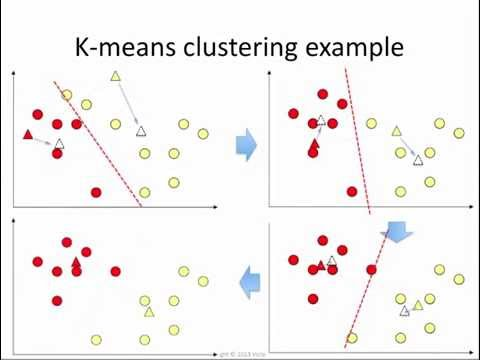
\includegraphics[width=0.8\textwidth]{proceso_kmeans}
	\end{center}
	\begin{center}
		\vskip -0.5cm
		\caption{\small{Proceso K-means.}}
		{\small{Fuente: }}
	\end{center}
\end{figure}


\subsubsection{Aplicaciones}

\begin{itemize}
	\item En marketing, para segmentar el mercado en pequeños grupos homogéneos donde realizar campañas publicitarias especificas.
	\item En biología, para dividir organismos en estructuras jerárquicas con el propósito de describir la diversidad biológica.
	\item En medicina, para diseñar tratamientos específicos para distintos grupos de riesgo.
	\item En psicología, para clasificar individuos en distintos tipos de personalidad, etc.
\end{itemize}

\subsection{Histograma}

\subsubsection{Definición}

Según \citep{histograma_unam} una histograma es una gráfica de la distribución de un conjunto de datos. Es un tipo especial de gráfica de barras y cada barra representa un subconjunto de los datos. Otra definición sostiene que un histograma es un gráfico de barras vertical que representa la distribución de frecuencias de un conjunto de datos \citep{histograma_aiteco}.

\vskip 1cm 
\subsubsection{Tipos}
Se agrupan los datos en clases, y se cuenta cuántas observaciones (frecuencia absoluta) hay en cada una de ellas. En algunas variables (variables cualitativas) las clases están definidas de modo natural, p.e sexo con dos clases: mujer, varón o grupo sanguíneo con cuatro: A, B, AB, O. En las variables cuantitativas, las clases hay que definirlas explícitamente (intervalos de clase) \citep{histograma_tipos}

\begin{itemize}
	\item \textbf{Simple:} Se representan los intervalos de clase en el eje de abscisas (eje horizontal) y las frecuencias, absolutas o relativas, en el de ordenadas (eje vertical).
	
%	\begin{figure}[ht]
%		\begin{center}
%			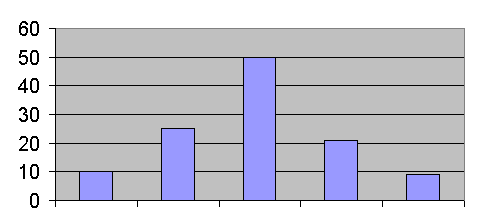
\includegraphics[width=0.8\textwidth]{histograma_simple}
%		\end{center}
%		\begin{center}
%			\vskip -0.5cm
%			\caption{\small{Histograma simple.}}
%			{\small{Fuente: \citep{histograma_tipos}}}
%		\end{center}
%	\end{figure}
	
	\item \textbf{Por grupos:} Se representan simultáneamente los histogramas de una variable en dos situaciones distintas.
	
	\item \textbf{Dirigido:} Se representan dos histogramas de la misma variable en dos situaciones distintas.
	
	\item \textbf{Estratificado:} Se representan el conjunto dividido en subconjuntos, a cada subconjunto se le denomina estrato.
	
\end{itemize}

\vskip 1cm 
\subsubsection{Aplicaciones}
\cite{histograma_tipos} nos indica las siguientes utilidades.
\begin{itemize}
	\item Proporciona, mediante el estudio de la distribución de los datos, un excelente punto de partida para formular hipótesis acerca de un funcionamiento insatisfactorio.
	\item El histograma es especialmente útil cuando se tiene un amplio número de datos que es preciso organizar, para analizar más detalladamente o tomar decisiones sobre la base de ellos.
	\item Es un medio eficaz para transmitir a otras personas información sobre un proceso de forma precisa.
	\item Permite la comparación de los resultados de un proceso con las especificaciones previamente establecidas para el mismo. Ayuda a determinar si el proceso satisface los requisitos del cliente.
	\item Hace posible determinar si ha habido cambios en un proceso.
	
\end{itemize}


\subsection{Predicción}

\subsubsection{Definición}

El término predicción puede referirse tanto a la acción y al efecto de predecir como a las palabras que manifiestan aquello que se predice; en este sentido, predecir algo es anunciar por revelación, ciencia o conjetura algo que ha de suceder \citep{rae_prediccion}.
\vskip 0.2cm 
Predicción es una expresión que anticipa aquello que "supuestamente" va a suceder. Se puede predecir algo a partir de conocimientos científicos, revelaciones de algún tipo, hipótesis o indicios.

\subsubsection{Tipos}

\begin{description}
	\item [Científica:]
	\vskip 0.1cm 
	La predicción constituye una de las esencias claves de la ciencia, de una teoría científica o de un modelo científico. Así, el éxito se mide por el acierto que tengan sus predicciones \citep{mora_prediccion}.
	\vskip 0.1cm 
	La  predicción  en  el  contexto  científico  es  una  declaración  precisa  de  lo  que  ocurrirá  en determinadas  condiciones  especificadas.  Se  puede  expresar  a  través  del  silogismo:  "Si  A  es cierto, entonces B también será cierto".
	\vskip 0.1cm 
	El método científico concluye con la prueba de afirmaciones que son consecuencias lógicas de las teorías científicas. Generalmente esto se hace a través de experimentos que deben poder repetirse o mediante estudios observacionales rigurosos.
	\vskip 0.1cm 
	Una teoría científica cuyas aseveraciones no son corroboradas por las observaciones, por las pruebas o por experimentos probablemente será rechazada.
	 
	\item [Predicción no científica:]
	\vskip 0.1cm 
	Los para-psicólogos y clarividentes, por su parte, apelan a pseudocientíficas para realizar predicciones. Estas personas dicen tener la posibilidad de conocer el futuro a partir de percepciones que reciben por sentidos que no son los cinco habituales (vista, olfato, gusto, oído y tacto). También hay sujetos que afirman recibir información por parte de entidades superiores(como dioses) para realizar sus predicciones \citep{julian_maria}
	\vskip 0.1cm 
	En estos casos, las predicciones no tienen ningún sustento lógico, por lo que creer en ellas suele ser una cuestión de fe o depender de la susceptibilidad de la persona.
	
\end{description}	
	

\subsection{Probabilidad}

\subsubsection{Definición}

La probabilidad es una medida de la certidumbre asociada a un suceso o evento futuro y suele expresarse como un número entre 0 y 1 (entre 0 \% y 100 \%). 
\vskip 0.1cm 
Una forma tradicional de estimar algunas probabilidades sería obtener la frecuencia de un acontecimiento determinado mediante la realización de experimentos aleatorios, de los que se conocen todos los resultados posibles, bajo condiciones suficientemente estables. Un suceso puede ser improbable (con probabilidad cercana a cero), probable (probabilidad intermedia) o seguro (con probabilidad uno) \citep{loeve}.

\subsubsection{Teoria de la probabilidad}

Según \citep{alvarez_rojas} la probabilidad \(p\) de que suceda un evento \(S\) de un total de \(n\) casos posibles igualmente probables es igual a la razón entre el número de ocurrencias \(h\) de dicho evento (casos favorables) y el número total de casos posibles \(n\).

\begin{align*}
p = Prob(S) = \frac{h}{n}\\
\end{align*}

La probabilidad es un número (valor) que varia entre 0 y 1. Cuando el evento es imposible se dice que su probabilidad es 0, si el evento es cierto y siempre tiene que ocurrir su probabilidad es 1.
La probabilidad de no ocurrencia de un evento está dada por \(q\), donde:
\begin{align*}
p = Prob(noS) = 1 - \frac{h}{n}\\
\end{align*}


\subsubsection{Teoría de bayes}

El teorema de Bayes, en la teoría de la probabilidad, es una proposición planteada por el matemático inglés Thomas Bayes (1702-1761) \citep{bayes} y publicada póstumamente en 1763, que expresa la probabilidad condicional de un evento aleatorio A dado B en términos de la distribución de probabilidad condicional del evento B dado A y la distribución de probabilidad marginal de sólo A.
\vskip 0.1cm 
Las probabilidades Bayesianas se utilizan para encontrar la distribución de probabilidad condicional de un evento dados otros eventos , debido a su naturaleza se puede implementar al razonamiento bajo incertidumbre, los primeros estudios estaban basados en encontrar los errores sistemáticos en la estimación de probabilidades apoyados por la heurística, básicamente se da el análisis de la información que se utiliza para determinar la incertidumbre de la misma al realizar razonamientos probabilísticos, y encontrar el nivel de validez de los resultados obtenidos bajo esta perspectiva.

{\bf Formula de bayes:}\par

Con base en la definición de Probabilidad condicionada \citep{bayes_formula} se obtiene la Fórmula de Bayes, también conocida como la Regla de Bayes.
\vskip 0.5cm 
Sea ${ A 1 , A 2 , . . . , A i , . . . , A n }$ un conjunto de sucesos mutuamente excluyentes y exhaustivos, y tales que la probabilidad de cada uno de ellos es distinta de cero $(0)$. Sea B un suceso cualquiera del que se conocen las probabilidades condicionales $P ( B | A i )$. Entonces, la probabilidad $P ( A i | B )$ viene dada por la expresión: 

\[ P ( A i | B )  = \frac{P ( B | A i ) P ( A i )} {P ( B )} \]

{\bf Donde:}\par

\begin{description}
	\item[$P ( A i )$] son las probabilidades a priori.
	\item[$P ( B | A i )$] es la probabilidad de $B$ en la hipótesis $( A i )$
	\item[$P ( A i | B )$] son las probabilidades a posteriori. 
\end{description}

\subsection{Pregunta de opción múltiple}

La pregunta de opción múltiple o de selección múltiple o multi-opción es una forma de evaluación por la cual se solicita a los encuestados o examinados seleccionar una o varias de las opciones de una lista de respuestas.
\vskip 1cm 
Este tipo de pregunta es usado en evaluaciones educativas (en lo que popularmente se llaman exámenes tipo test), en elecciones (para escoger entre múltiples candidatos o partidos políticos diferentes), en los cuestionarios para estudios de mercado, encuestas, estadística y muchas otras áreas.

\begin{figure}[ht]
	\begin{center}
		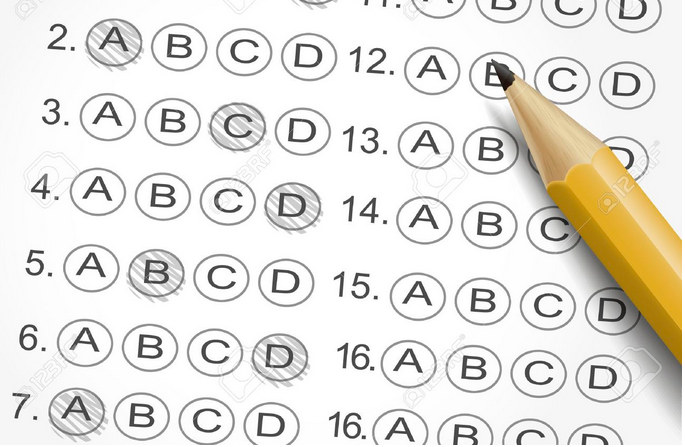
\includegraphics[width=0.8\textwidth]{pregunta_opcion_multiple}
	\end{center}
	\begin{center}
		\vskip -0.5cm
		\caption{\small{Hoja de respuestas de opción múltiple.}}
		{\small{Fuente: \citep{pregunta_opcion_multiple}}}
	\end{center}
\end{figure}
 
{\bf Formato:}\par

Un formato típico puede ser el de un enunciado seguido de una pregunta al respecto. El examinador ofrecerá normalmente de entre tres a cinco respuestas típicamente ( a, b, c, d, e) de las cuales solamente una va a ser la respuesta correcta (la mejor respuesta) mientras las restantes respuestas serán los distractores \citep{salkind}.
\vskip 1cm 


\subsection{Prototipo de software}

\subsubsection{Definición}

En Ingeniería de software un prototipo es una representación limitada del diseño de un producto que permite a las partes responsables de su creación experimentar su uso \citep{pressman_troya}, el prototipo debe ser construido en poco tiempo, usando los programas adecuados y no se debe utilizar muchos recursos.
\vskip 0.3cm
El diseño rápido se centra en una representación de aquellos aspectos del software que serán visibles para el cliente o usuario final. Este diseño conduce a la construcción de un prototipo, el cual es evaluado por el cliente para una retroalimentación; gracias a ésta se refinan los requisitos del software que se desarrollará. La interacción ocurre cuando el prototipo se ajusta para satisfacer las necesidades del cliente. Esto permite que al mismo tiempo el desarrollador entienda mejor lo que se debe hacer y el cliente vea resultados a corto plazo \citep{pressman_troya}.


\subsubsection{Ventajas}

\begin{itemize}
	\item Este modelo es útil cuando el cliente conoce los objetivos generales para el software, pero no identifica los requisitos detallados de entrada, procesamiento o salida.
	\item También ofrece un mejor enfoque cuando el responsable del desarrollo del software está inseguro de la eficacia de un algoritmo, de la adaptabilidad de un sistema operativo o de la forma que debería tomar la interacción humano-máquina.
	\item Se puede reutilizar el código.
\end{itemize}

\subsubsection{Aplicación web}
En la ingeniería de software se denomina aplicación web a aquellas herramientas que los usuarios pueden utilizar accediendo a un servidor web a través de Internet o una intranet mediante un navegador. En otras palabras, es una aplicación software que se codifica en un lenguaje soportado por los navegadores web \citep{mora}.

\subsubsection{LAMP}

LAMP es el acrónimo usado para describir un sistema de infraestructura de internet que usa las siguientes herramientas:

\begin{itemize}
	\item Linux, el sistema operativo.
	\item Apache, el servidor web.
	\item MySQL/MariaDB, el gestor de bases de datos.
	\item Perl, PHP, o Python, los lenguajes de programación. 
\end{itemize}

La combinación de estas tecnologías es usada principalmente para definir la infraestructura de un servidor web, utilizando un paradigma de programación para el desarrollo \citep{apache}.
\vskip 0.3cm
A pesar de que el origen de estos programas de código abierto no han sido específicamente diseñado para trabajar entre sí, la combinación se popularizó debido a su bajo coste de adquisición y ubicuidad de sus componentes (ya que vienen pre-instalados en la mayoría de las distribuciones linux). Cuando son combinados, representan un conjunto de soluciones que soportan servidores de aplicaciones.

\subsubsection{Software}

\begin{itemize}
	\item \textbf{Linux:} Linux es un núcleo de sistema operativo libre tipo Unix.
	\item \textbf{Apache HTTP Server:} El servidor HTTP Apache es un servidor web libre y de código abierto, el más popular en cuanto a uso, sirviendo como plataforma de referencia para el diseño y evaluación de otros servidores web.
	\item \textbf{MySQL:} MySQL es un Sistema de Gestión de Bases de Datos (SGBD) relacional, que por lo tanto utiliza SQL, multihilo y multiusuario del que se estiman más de un millón de instalaciones.
	\item \textbf{PHP:} PHP (acrónimo recursivo de "PHP: Hypertext Preprocessor") es un lenguaje de programación diseñado para producir sitios web dinámicos. PHP es utilizado mayormente en aplicaciones del lado del servidor.
\end{itemize}

\begin{figure}[ht]
	\begin{center}
		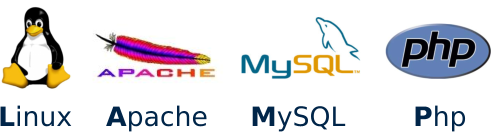
\includegraphics[width=0.8\textwidth]{LAMP_software}
	\end{center}
	\begin{center}
		\vskip -0.5cm
		\caption{\small{Software usado en LAMP.}}
		{\small{Fuente: }}
	\end{center}
\end{figure}

\section{Método de la investigación}

\subsection{Metodología de la investigación}

Se realizará una investigación aplicada, con una investigación cuantitativa, ya que se planea verificar con porcentajes y gráficos la cantidad de predicciones acertadas y al final verificar si las predicciones son correctas o no.
\vskip 0.1cm 
Para las pruebas se aplicara el estudio de caso con una sola medición en cual consiste en administrar un estimulo o tratamiento a un grupo y después aplicar una medición de una o mas variables para observar cual es el nivel del grupo en estas variables [AGREGAR CITA]. El diseño se diagrama de la siguiente manera: 

\[ G  - - > X - - > O \]

\vskip 0.1cm 
Donde
\vskip 0.1cm 

\begin{itemize}
	\item [$G =$] Grupo de sujetos.
	\item [$X =$] Tratamiento, estimulo o condición experimental.
	\item [$O =$] Medición de los sujetos de un grupo.
\end{itemize}

\subsection{Población}

La población para el presente estudio son las preguntas de la evaluación, para medir el nivel de inglés, de los 17 estudiantes de la sección 602 del centro de idiomas El Cultural. Esta evaluación consta de 18 preguntas y fue aplicada en Diciembre del 2016.

\subsection{Muestra}

Dado que cada evaluación consta de 18 preguntas y hay 17 estudiantes en la sección, en total tendremos 306 items de preguntas. Para esto se usara un muestreo aleatorio simple para poblaciones finitas con un nivel de confianza del 95 \%  y un error de muestreo del 5\%. [AGREGAR CITA]

\[ n  = \frac{ N * p^{2} z^{2} } { (N - 1) * e^{2} + p^{2} z^{2} } \]

\vskip 0.1cm 
Donde
\vskip 0.1cm 

\begin{itemize}
	\item [$n =$] Grupo de sujetos.
	\item [$N =$] Tamaño de la población. En este caso 170.57.
	\item [$z =$] Coeficiente de confiabilidad (1,96), lo que representa el 95 \% de confianza.
	\item [$p =$] Desviación estándar de la población. 50 \% = 0.50 (caso más desfavorable, desconocido).
	\item [$z =$] Margen de error 5 \% = (0,05).
\end{itemize}

Aplicando la formula obtenemos que la muestra es de tamaño 170.57 = 171. La cual nos da un promedio de 10 preguntas por estudiante.


\subsection{Variable de estudio}

%Tipo de variables 				Nombre de la variable 							Indicadores

%Independiente Técnicas     Técnicas de aprendizaje no supervisado       Analisis del algoritmo

%Dependiente       Predicción de la respuesta correcta de una            Grado de acierto del resultado   
%				  pregunta de opción múltiple	

\subsection{Instrumento de recolección de datos}

\begin{itemize}
	\item Formato para registrar las notas de los estudiantes. Apéndice B
	\item Formato para registrar las respuestas de los estudiantes. Apéndice C
	\item Prototipo de software web donde se ingresaran los datos.
\end{itemize}

\subsection{Procedimiento}

\begin{enumerate}
	\item Formulación del problema principal de la investigación, justificando su importancia.
	\item Búsqueda del material bibliográfico de los diferentes temas necesarios para la elaboración de la investigación, tales como aprendizaje automático no supervisado, probabilidades, estadísticas, desarrollo web, entre otros.
	\item Estudio y análisis de los algoritmos de aprendizaje automático no supervisado.
	\item Estudio de modelos probabilísticos y estadísticos que contribuyan con el tema de predicciones.
	\item Desarrollo del algoritmo de aprendizaje automático no supervisado.
	\item Desarrollo del prototipo de software web.
	\item Elección de los datos de prueba.
	\item Testear, validar y documentar los resultados de la investigación.
\end{enumerate}




\chapter{Tema central de la tesis}

Basados en los conceptos discutidos en los capítulos 1 y 2. Se procederá a realizar el modelamiento de todo el proceso de predicción de la respuesta correcta, el desarrollo del algoritmo y de cada paso del proceso hasta llegar a resultado final.

\section{Desarrollo del algoritmo de aprendizaje no supervisado K-means} 

\subsection{Implementación}

\subsubsection{Diagrama de flujo}

El algoritmo tiene diferentes pasos en su proceso los cuales vemos en la \textbf{figura \ref{fig:steps_kmeans}}

\begin{figure}[H]
	\begin{center}
		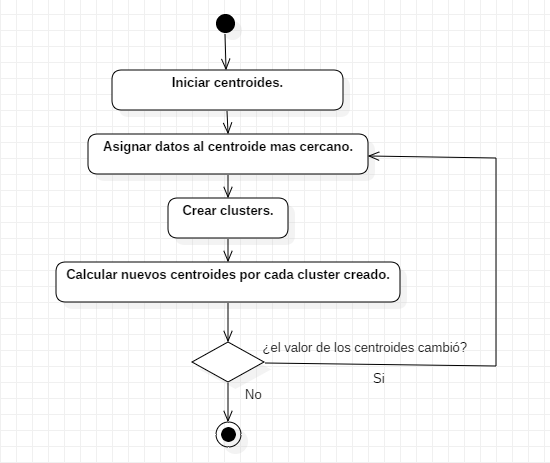
\includegraphics[width=0.8\textwidth]{steps_kmeans}
	\end{center}
	\begin{center}
		\vskip -0.5cm
		\caption{\label{fig:steps_kmeans}\small{Diagrama de actividades/flujo algoritmo Kmeans.}}
		{\small{Fuente: Propia }}
	\end{center}
\end{figure}

\subsubsection{Pseudocodigo}
Se muestra los pasos del \textbf{ algoritmo \ref{alg:algorithm_kmeans} } representado en pseudocodigo.

\begin{algorithm}[H]
\begin{algorithmic}[1]
		\REQUIRE Grupo de datos, Número de clusters.  % Entrada
		%\label{alg:algorithm_kmeans}
		\ENSURE Centroides, Datos con sus respectivos clusters.                                                       % Salida
		
		\STATE Iniciar centroides.
					
		\STATE Asignar datos al centroide. \label{marker}
			
		\STATE Crear clusters.
			
		\STATE Calcular nuevos centroides por cada cluster creado.
			
		\IF {El valor de los centroides cambió}
			\STATE {\bf Goto} [ Paso 3]
		\ENDIF
			
		\RETURN  Centroides, Datos con sus respectivos clusters.
		
		\begin{center}
		    \vskip -0.5cm
	    	\caption{\label{alg:algorithm_kmeans}\small{Pseudocodigo  Kmeans.}}
	    \end{center}

\end{algorithmic}
\end{algorithm}


\subsection{Proceso}

En esta sección se muestra el proceso que sigue K-means en las \textbf{figuras \ref{fig:step_kmeans_1}, \ref{fig:step_kmeans_2}, \ref{fig:step_kmeans_3},\ref{fig:step_kmeans_final}} a través de todas las iteraciones que realiza hasta lograr que los grupos se puedan estabilizar en ese momento las iteraciones finalizan.

\begin{figure}[H]
	\begin{center}
		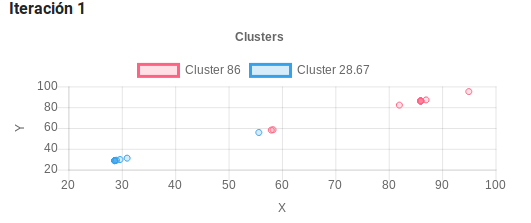
\includegraphics[width=0.8\textwidth]{step_kmeans_1}
	\end{center}
	\begin{center}
		\vskip -0.5cm
		\caption{\label{fig:step_kmeans_1}\small{Grupos obtenidos en la iteración 1 .}}
		{\small{Fuente: Propia. }}
	\end{center}
\end{figure}

\begin{figure}[H]
	\begin{center}
		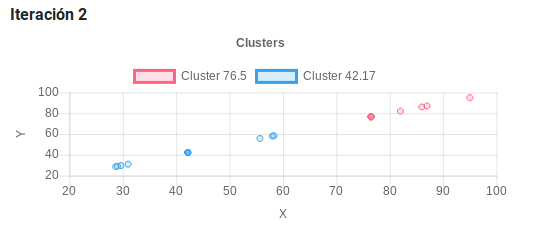
\includegraphics[width=0.8\textwidth]{step_kmeans_2}
	\end{center}
	\begin{center}
		\vskip -0.5cm
		\caption{\label{fig:step_kmeans_2}\small{Grupos obtenidos en la iteración 2 .}}
		{\small{Fuente: Propia. }}
	\end{center}
\end{figure}

\begin{figure}[H]
	\begin{center}
		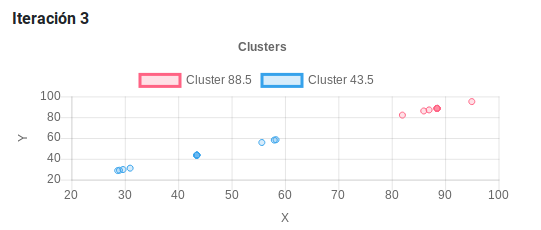
\includegraphics[width=0.8\textwidth]{step_kmeans_3}
	\end{center}
	\begin{center}
		\vskip -0.5cm
		\caption{\label{fig:step_kmeans_3}\small{Grupos obtenidos en la iteración 3 (Final) .}}
		{\small{Fuente: Propia. }}
	\end{center}
\end{figure}

\begin{figure}[H]
	\begin{center}
		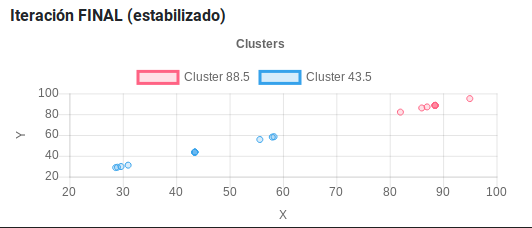
\includegraphics[width=0.8\textwidth]{step_kmeans_final}
	\end{center}
	\begin{center}
		\vskip -0.5cm
		\caption{\label{fig:step_kmeans_final}\small{Grupos obtenidos en la iteración FINAL (estabilizado) .}}
		{\small{Fuente: Propia. }}
	\end{center}
\end{figure}

\section{Histograma}

\subsection{Modelado}

\subsubsection{Diagrama de flujo}

El histograma tiene diferentes pasos en su proceso los cuales vemos en la \textbf{ figura \ref{fig:steps_histogram}}

\begin{figure}[H]
	\begin{center}
		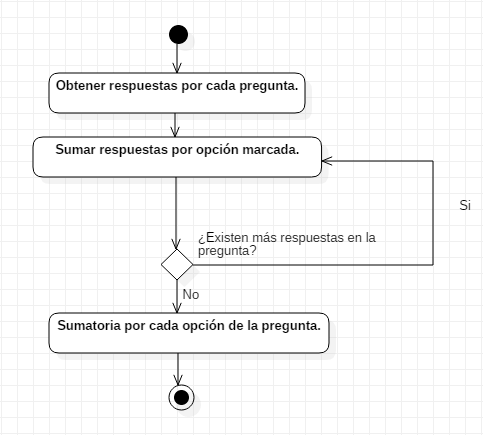
\includegraphics[width=0.8\textwidth]{steps_histogram}
	\end{center}
	\begin{center}
		\vskip -0.5cm
		\caption{\label{fig:steps_histogram}\small{Diagrama de actividades/flujo Histograma. }}
		{\small{Fuente: Propia.}}
	\end{center}
\end{figure}


\subsubsection{Pseudocodigo}
Los pasos representados en \textbf{ algoritmo \ref{alg:pseudocode_histogram}}.

\begin{algorithm}[H]
	\begin{algorithmic}[2]
		\REQUIRE Respuestas de una pregunta.  % Entrada
		\ENSURE Sumatoria por cada opción de la pregunta .                                                       % Salida
		
		\STATE Obtener respuestas por pregunta.
		
		\STATE Sumar respuestas según la opción marcada. 
		
	
		\IF {Existen más respuestas en la pregunta}
		\STATE {\bf Goto} [ Paso 2]
		\ENDIF
		
		\RETURN  Sumatoria por cada opción de la pregunta.
		
		\begin{center}
			\vskip -0.5cm
			\caption{\label{alg:pseudocode_histogram}\small{Pseudocodigo del actividades/flujo histograma.}}
		\end{center}
		
	\end{algorithmic}
\end{algorithm}


\subsection{Proceso}

En esta sección se muestra el proceso donde se genera el histograma, en las \textbf{figuras \ref{fig:step_kmeans_1}, \ref{fig:step_kmeans_2}, \ref{fig:step_kmeans_3},\ref{fig:step_kmeans_final}} a través de todas las iteraciones que realiza hasta lograr que los grupos se puedan estabilizar en ese momento las iteraciones finalizan.

\begin{figure}[H]
	\begin{center}
		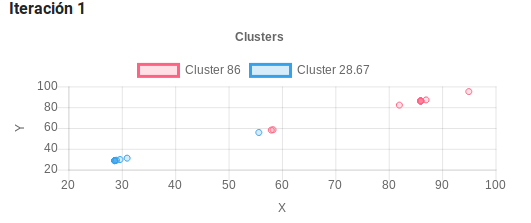
\includegraphics[width=0.8\textwidth]{step_kmeans_1}
	\end{center}
	\begin{center}
		\vskip -0.5cm
		\caption{\label{fig:step_kmeans_1}\small{Grupos obtenidos en la iteración 1 .}}
		{\small{Fuente: Propia. }}
	\end{center}
\end{figure}









\section{Prototipo de aplicación web} 

\subsection{Modelamiento del proceso}

En esta sección vemos los pasos para poder realizar todo el proceso de la predicción de la respuesta correcta usando el prototipo desarrollado. En la figura \ref{fig:flow_chart_all_process} se muestra el diagrama de actividades de los procesos, la interaccion entre el usuario y el prototipo de aplicación web.

\begin{figure}[ht]
	\begin{center}
		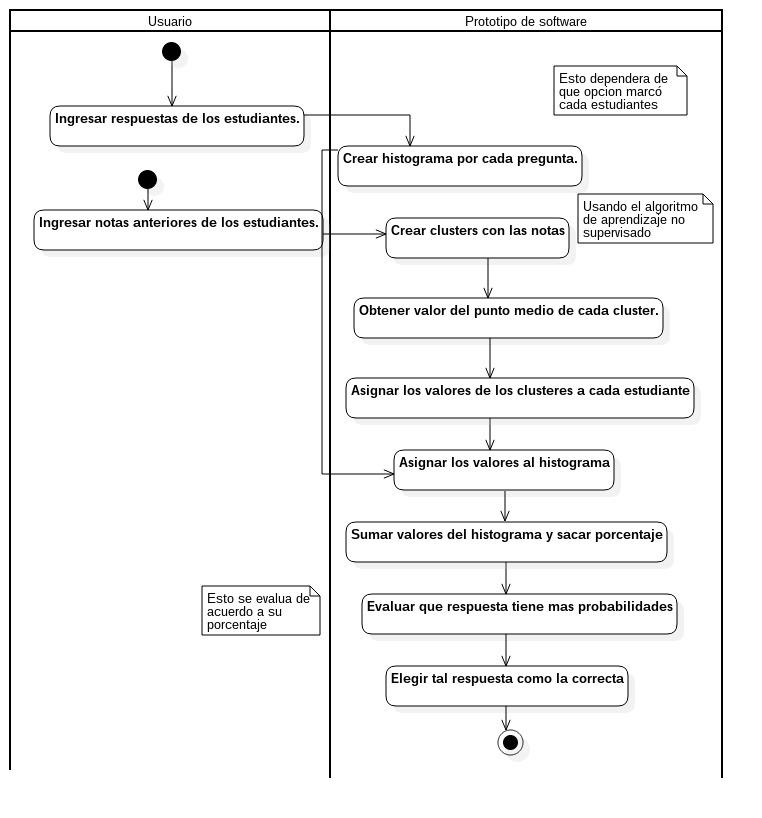
\includegraphics[width=0.8\textwidth]{flow_chart_all_process}
	\end{center}
	\begin{center}
		\vskip -0.5cm
		\caption{\small{Diagrama de actividades de todo el proceso.}}
		{\small{Fuente: }}
	\end{center}
\end{figure}


\subsection{Desarrollo}

El desarrollo del prototipo se realizo bajo un entorno Linux, usando Apache como servidor web, PHP como el lenguaje de servidor y HTML para la vistas. En la Figura 3.7 podemos ver la pantalla principal del prototipo donde muestra las diferentes opciones habilitadas. (MOSTRAR PANTALLA PRINCIPAL)

\subsection{Base de datos}
Algunos de los datos que se necesitan debían de ser permanentes, por lo cual se creo una pequeña base de datos para almacenarlos En la figura 3.8 vemos el diagrama relacional de la base de datos. (MOSTRAR DIAGRAMA DE LA BDD)


\section{Proceso para realizar la predicción} 

\subsection{Ejecutar K-means}

En la figura 3.9 se muestra los resultados de ejecutar K-means. Esta ejecución nos da como resultado los clusters ordenados. Mostrando los datos de los estudiantes, el promedio de sus notas, el cluster al que pertenecen y el valor de estos clusters.
(MOSTRAR RESULTADO DE LA EJECUCION KMEANS)

\subsection{Histograma por pregunta}

Por cada pregunta se obtiene cuantos estudiantes marcaron cada uno de las opciones, creando un histograma usando las respuestas por cada pregunta.

\subsubsection{Modelado}

El proceso del crear el histograma tiene diferentes pasos los cuales vemos en la Figura 3.10 \ref{fig:steps_histogram_process}

\begin{figure}[ht]
	\begin{center}
		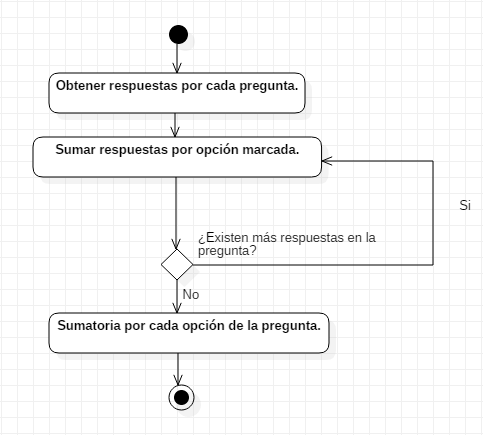
\includegraphics[width=0.8\textwidth]{steps_histogram}
	\end{center}
	\begin{center}
		\vskip -0.5cm
		\caption{\small{Pasos para el proceso del histograma.}}
		{\small{Fuente: Propia}}
	\end{center}
\end{figure}

\subsubsection{Modelado}

Se realizo la prueba de ejecución utilizando una pregunta de 4 opciones y con la respuesta de 7 estudiantes. En la figura 3.11 se muestra los resultados el histograma de una pregunta. En donde se muestra las opciones de la pregunta, el nombre los estudiantes que marcaron cada pregunta y el total de estudiantes por pregunta.
(MOSTRAR RESULTADO DEL HISTOGRAMA)

\subsection{Asignación valores de los clusters al histograma}

Después de haber obtenido el histograma de una pregunta, Se asigna el valor del cluster que pertenece a cada estudiante en el histograma, obteniendo la suma de ellos por cada opción. Luego se suman los resultados de todas las opciones para sacar un porcentaje por cada una y así la opción con mayor porcentaje sera elegida como la correcta. (EXPLICAR EL PROCESO)

\subsubsection{Modelado}

El proceso de asignar valores de los cluster al histograma tiene diferentes pasos los cuales vemos en la Figura \ref{fig:steps_asign_values_to_cluster}.

\begin{figure}[ht]
	\begin{center}
		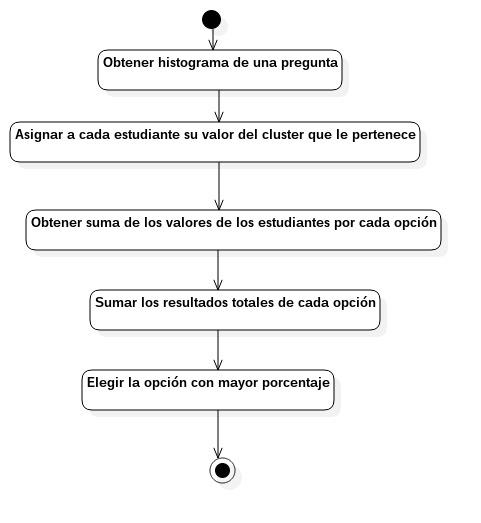
\includegraphics[width=0.8\textwidth]{steps_asign_values_to_cluster}
	\end{center}
	\begin{center}
		\vskip -0.5cm
		\caption{\small{Pasos para la asignación valores de los cluster al histograma.}}
		{\small{Fuente: Propia}}
	\end{center}
\end{figure}

\subsubsection{Resultado}

Se realizo la prueba de ejecución utilizando una pregunta de 4 opciones y con la respuesta de 7 estudiantes. En la figura 3.13 se muestra los resultados de la asignación valores de los 33cluster al histograma, mostrando también cual es la opción elegida como la correcta. En donde se muestra las opciones de la pregunta, el nombre los estudiantes que marcaron cada pregunta,
el total de estudiantes por pregunta, la suma de los valores de los clusters de cada estudiante por cada opción, el porcentaje de cada opción de la suma de los clusters y cual es la opción correcta según la que tiene mas porcentaje de la suma de los valores de los clusters. (MOSTRAR CAPTURA Y ARREGLAR TEXTO)


\section{Comparación de resultados} 

Las respuestas predecidas de cada preguntas se comparan con las respuestas correctas para poder obtener cuantas han sido predecidas correctamente.

\subsection{Resultado}

Se realizo la prueba de ejecución con 3 preguntas. La figura 3.14 muestra primero un resumen de cuantas predicciones de las respuestas de las preguntas fueron correctas y cuantas no Después muestra la lista de preguntas con su respuesta predecida, la respuesta que es la correcta y una opción que muestra si las 2 respuestas coinciden.
(MOSTRAR DONDE SE COMPRAN LAS PREGUNTAS)





















\section{Proceso de modelamiento} 

{\bf Ejemplo:}\par

La planificación y modelamiento del sistema de logística reversa de una área urbana es una fase importante y estratégica, para obtener en el futuro óptimos resultados en el proceso de gerenciamiento y operación del sistema reverso de RSU. El modelamiento permite determinar la localización de las estaciones de colecta y de unidades especiales necesarias, asi como el flujo que será movido a los largo de la red permitiendo dimensionar todo el sistema y sus componentes (Figura 3.1).
\vskip 0.3cm
\begin{figure}[ht]
\begin{center}
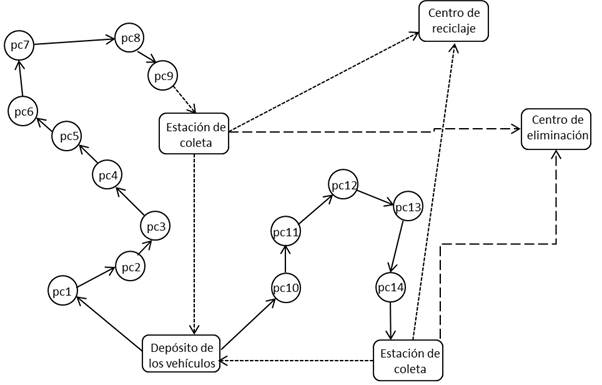
\includegraphics[width=.6\textwidth]{Figura3}
\end{center}
\begin{center}
\vskip -0.5cm
\caption{\small{Esquema del proceso de colecta y transporte de RSU.}}
{\small{Fuente: Elaboración propia}}
\end{center}
\end{figure}

\subsection{Proceso de ruteo}

\section{Implementación} 
























\chapter{Resultados y discusión de la tesis}


Al culminar con la investigación se llegaron a resultados interesantes del punto de vista tanto teórico como computacional. Estos resultados muestran que se contrasta la hipótesis planteada durante el proceso de elaboración del plan de investigación, es decir, que se logró demostrar la relación entre las variables de estudio formuladas en la investigación.

\section{Teóricos}

\section{Computacionales}




\chapter{Consideraciones finales}


\section{Conclusiones}

{\bf Ejemplo}\\
La investigación bibliográfica revela que realmente existe una preocupación de los gobiernos con el destino final de los residuos sólidos, con el objetivo de preservar la salud de la población y el medio ambiente urbano y rural. Por ejemplo, se observa la creación de la Ley 12305. Sin embargo existe una laguna entre las metas propuestas en la ley con las metas reales de los gobiernos locales. Eso se debe a la falta de una buena estructura organizacional, gerencial y operacional de los gobiernos locales capaz de atender las demandas locales y las necesidades de la población.
\vskip 0.3cm
La falta de cuadros especializados, tanto en los gobiernos centrales como locales, para realizar la planificación y modelamiento de una red logística reversa puede ser compensada con la contribución de los investigadores que actúan en ese campo del conocimiento. Es muy difícil la formación de un equipo que tenga todo el conocimiento en las áreas de ciencia de la computación, de geo procesamiento, de modelamiento matemático y de logística reversa, entre otras. Esa es una de las principales justificativas que los gobiernos, argumentan a la falta de planificación de una red logística reversa que funciones eficaz y eficientemente. 
\vskip 0.3cm
Por lo tanto, como quedó demostrado a lo largo de este trabajo, es posible realizar el modelamiento matemático para este tipo de problema con baja inversión, así como aplicarlo en varias regiones sin necesidad de grandes cambios en el modelamiento propuesto. El modelo propuesto calcula los flujos en la red logística reversa, permitiendo dimensionar la cantidad y capacidad de las unidades productivas y de los vehículos. 
\vskip 0.3cm
...


\section{Trabajos futuros}



\cleardoublepage
\addcontentsline{toc}{chapter}{Bibliografía}
\bibliographystyle{apalike}  % estilo de la bibliografía APA.
\bibliography{Bibliografia}   % Bibliografia.bib es el fichero donde está salvada la bibliografía.


                % Capitulos de la tesis

\appendix
\chapter{Primer apendice}
hola como estas
\chapter{Segundo apendice}
si te escucho
\chapter{Tercer apendice}
sdsdsd


\chapter*{\hspace*{1cm} Declaración jurada y autorización}

\addtocontents{toc}{\vspace{2em}}
Los autores suscritos de la tesis: \\ 
{\small escribir nombre de la tesis} \\
declaramos su originalidad y autorizamos su publicación en el repositorio digital institucional y repositorio RENATI-SUNEDU, con el siguiente tipo de acceso: NOTA: Elegir un tipo de acceso

\begin{enumerate}
\item[a)] Acceso abierto: SI/NO
\item[b)] Acceso restringido (datos del autor y resumen del trabajo): SI/NO
\item[c)] No autorizo su publicación: 
\end{enumerate}
Si eligió la opción restringido  o NO autoriza su publicación sírvase justificar: 
%\vskip 0.3cm

El equipo investigador integrado por: \\
\hspace{-0.5cm}
\begin{tabular}{|c|c|c|c|c|}
\hline 
Apellidos y nombres & Condición de docente/estudiante & Código docente/Num. mat. & Autor/asesor \\ \hline 
Peche Perlado Edgar & Estudiante & 10101010 & Autor  \\ \hline 
Pérez Yon Manuel & Estudiante & 10101010 & Autor  \\ \hline 
Rodríguez M. José & Docente & 4010 & Asesor  \\ \hline 
\end{tabular} 
\vskip 1.2cm
\hspace{0.7cm}Edgar\hspace{.1cm}M.\hspace{.1cm} Peche\hspace{.1cm}Perlado 
\hspace{4cm}Manuel\hspace{.1cm}E.\hspace{.1cm} Pérez\hspace{.1cm}Yon \\
\hspace*{2.6cm} DNI:  \hspace*{6.6cm}DNI:


\vskip 0.6cm
\begin{center}
José  \hspace{.1cm}A.\hspace{.1cm} Rodríguez\hspace{.1cm}Melquiades\\
 DNI:
\end{center}

           % Apendice

\end{document}






